\documentclass[11pt]{article}
\usepackage[final]{acl}   % EMNLP 2026 demo = single-blind (authors shown). Switch to [review] if needed.
\usepackage{times}
\usepackage{latexsym}
\usepackage[T1]{fontenc}
\usepackage[utf8]{inputenc}
\usepackage{microtype}
\usepackage{graphicx}
\usepackage{booktabs}
\usepackage{enumitem}
\usepackage{amssymb}
\usepackage{xcolor}
\usepackage{url}

\newcommand{\yes}{\textcolor{green!55!black}{\checkmark}}
\renewcommand{\mid}{\textcolor{orange!85!black}{$\sim$}}
\newcommand{\no}{\textcolor{red!70!black}{$\times$}}

\title{PolyInterview: A Deployed Multi-Agent System for\\ Explainable, Multimodal Mock-Interview Feedback}

% Single-blind, non-anonymous. TODO(authors): confirm exact emails for co-authors before submission.
\author{
  Zhiyuan Wen$^{1}$, Jiannong Cao$^{1}$, Zijian Wang$^{1}$, Chen Chen$^{1}$, \\
  Xiaoyun Liu$^{1}$, Jianing Yin$^{1}$, Zhuo Li$^{2}$ \\[3pt]
  \normalfont $^{1}$Department of Computing, The Hong Kong Polytechnic University, Hong Kong, China \\
  \normalfont $^{2}$School of Artificial Intelligence, Chongqing University of Posts and Telecommunications, China \\[3pt]
  \normalfont\texttt{\{zyuanwen, jiannong.cao, zi-jian.wang\}@polyu.edu.hk} \\
  \normalfont\texttt{\{chen03.chen, xiaoyun.liu, jianing-laetitia.yin\}@connect.polyu.hk} \\
  \normalfont\texttt{cliff.zhuo.li@gmail.com}
}

\begin{document}
\maketitle

\begin{abstract}
Interview practice is scarce and expensive, and the feedback that decides a real hiring outcome (how you reason, how you speak, how you carry yourself) is exactly what solo practice cannot give back. Existing AI interview tools tailor only the first question, walk a fixed list without follow-ups, score text alone, and rarely tie a number to a reason. We present \textbf{PolyInterview}, a publicly deployed multi-agent system in which a student rehearses a complete, embodied mock interview with a lip-synced digital-human interviewer that adapts its follow-ups, and then receives feedback that is multi-dimensional and \emph{traceable}. A planner agent assembles a personalized question list from the job description and CV; an interviewer agent decides follow-ups from a live check of each answer's consistency, clarity, and relevance; and four feature agents run in parallel over text, audio, and video, producing thirteen behavioral features that a three-layer architecture rolls up into ten competency aspects and two proficiency tracks, grounded in the established KSA and STAR hiring frameworks. The system has served students across six institutions and is live at \url{https://polyinterview.comp.polyu.edu.hk/}, with a $\leq$2.5-minute screencast walking through one end-to-end session. Reanalyzing a cleaned 120-session deployment corpus, we find that the per-feature architecture does something benchmarks hide: it makes its own failure modes legible. Most sharply, the non-verbal evaluator silently fails on roughly a third of recorded answers, which we report as both a finding and an agenda for validation.
\end{abstract}

\section{Introduction}
Hiring has tightened and shifted toward skills-based selection that probes both soft and hard skills \emph{inside} the interview. Good practice has not kept up. Real interviews are too rare to learn from, and an expert mock interview runs on the order of US\$150--200 per session and does not scale during peak recruiting. Practicing alone is worse than it looks: it never produces the probing follow-up that exposes a thin answer, and it gives no feedback on the voice and body language that interviewers read within the first minute. The cost is real: structured interviews predict job performance with a validity near $0.51$ \citep{schmidt1998validity}, and impressions formed from a few seconds of behavior already track the final decision \citep{ambady1992thin}. A candidate who cannot rehearse those signals is rehearsing the wrong thing.

AI is the natural response, and several products exist, but they share three gaps. \textbf{Personalization} stops early: question banks are generic, or only the opening question is tailored, with no reasoning over what the candidate just said. \textbf{Interaction} is shallow: a session advances through a fixed list whether an answer is sharp, vague, or self-contradictory, losing the multi-turn pressure of a real interview. \textbf{Assessment} is narrow and opaque: methods read the transcript and drop voice and non-verbal behavior, and even when a rubric is applied, its dimensions seldom map to any theory, so a score arrives without a reason a student can act on. The history here is cautionary: HireVue withdrew its facial-analysis feature in 2020 after sustained criticism. That makes \emph{explainable, advisory} non-verbal feedback the responsible target, not a reason to abandon the modality.

We organize the design around a frame from selection psychology: an offer is \textsc{Match} $\times$ \textsc{Convince}. \textsc{Match} is whether ability fits the role: the Knowledge, Skills, and Abilities (KSA) a recruiter looks for. \textsc{Convince} is whether the candidate communicates that fit. Because an offer is a product and not a sum, a useful system has to serve both sides in one loop. \textbf{PolyInterview} does so as a deployed, live system;\footnote{Live demo: \url{https://polyinterview.comp.polyu.edu.hk/}. Screencast ($\leq$2.5\,min, MPEG4) submitted separately.} to our knowledge it is among the first AI mock-interview platforms to put a digital-human interviewer and a theory-grounded, multimodal, explainable evaluation pipeline in a single end-to-end interaction. Our contributions:
\begin{enumerate}[noitemsep,topsep=2pt,leftmargin=*]
  \item A working, publicly available mock-interview \emph{system} with an embodied digital-human interviewer and complete, multi-stage interviews rather than one-off Q\&A (\S\ref{sec:system}).
  \item A multi-agent design in which a planner agent personalizes the question list and an interviewer agent generates follow-ups from a real-time answer check, extending personalization \emph{past} the first question with configurable difficulty (\S\ref{sec:system}).
  \item A three-layer, KSA$\times$STAR-grounded scoring pipeline with four parallel feature agents over text, audio, and video (13 features $\rightarrow$ 10 aspects $\rightarrow$ 2 tracks), where every score traces back to a behavioral signal (\S\ref{sec:scoring}).
  \item A real deployment and a reanalysis of a cleaned 120-session corpus that turns the architecture's traceability into a concrete, actionable finding about evaluator reliability, plus a validation plan (\S\ref{sec:deploy}--\S\ref{sec:eval}).
\end{enumerate}

\section{Related Work}
\label{sec:related}
\paragraph{Commercial AI interview tools.} Google Interview Warmup, Yoodli, Big Interview, HireVue, and Interviewing.io cover much of the practical market. Each solves part of the problem (delivery metrics, model answers, or human coaching), but as Table~\ref{tab:compare} lays out, none combines adaptive questioning, multimodal \emph{explainable} scoring, and a coherent multi-stage interview in one self-serve tool.

\paragraph{Automated video interviews.} Work in affective computing and industrial-organizational psychology predicts interview constructs from multimodal features \citep{naim2018automated,hemamou2019hirenet}, usually by extracting hand-engineered signals and regressing them onto recruiter ratings. These pipelines can be accurate, but they emit a score, not the evidence behind it, which limits their use as a \emph{learning} tool and complicates accountability; their reliability and validity are also uneven across constructs \citep{hickman2022automated}. We instead frame video evaluation as an evidence-based, explainable process rather than score regression, and ship that stance in a deployed, student-facing system.

\paragraph{Foundation models as evaluators.} Using language and vision-language models as judges is now common \citep{zheng2023judging} and carries known biases. We use such models not as black-box raters but as agents in a layered pipeline whose intermediate features and aspects are exposed to the user and bound to established hiring frameworks, so a judgment can be inspected and argued with.

\begin{table*}[t]
\centering\small
\begin{tabular}{lccccc}
\toprule
& \textbf{Adaptive} & \textbf{Theory-grounded} & \textbf{Multimodal} & \textbf{Multi-stage} & \textbf{Explainable} \\
& \textbf{follow-ups} & \textbf{feedback} & \textbf{(text/audio/video)} & \textbf{interview} & \textbf{\& traceable} \\
\midrule
Google Interview Warmup & \no & \mid & \mid & \no & \no \\
Yoodli & \no & \mid & \mid & \no & \no \\
Big Interview & \mid & \mid & \no & \no & \no \\
HireVue & \mid & \mid & \no\,(removed 2020) & \mid & \no \\
Interviewing.io (human) & \yes & \yes & --- & \yes & \mid \\
\textbf{PolyInterview (ours)} & \yes & \yes\,(KSA$\times$STAR) & \yes & \yes & \yes \\
\bottomrule
\end{tabular}
\caption{Positioning against representative interview-practice tools. \yes\ full, \mid\ partial, \no\ absent.}
\label{tab:compare}
\end{table*}

\section{System Overview}
\label{sec:system}

\begin{figure*}[t]
  \centering
  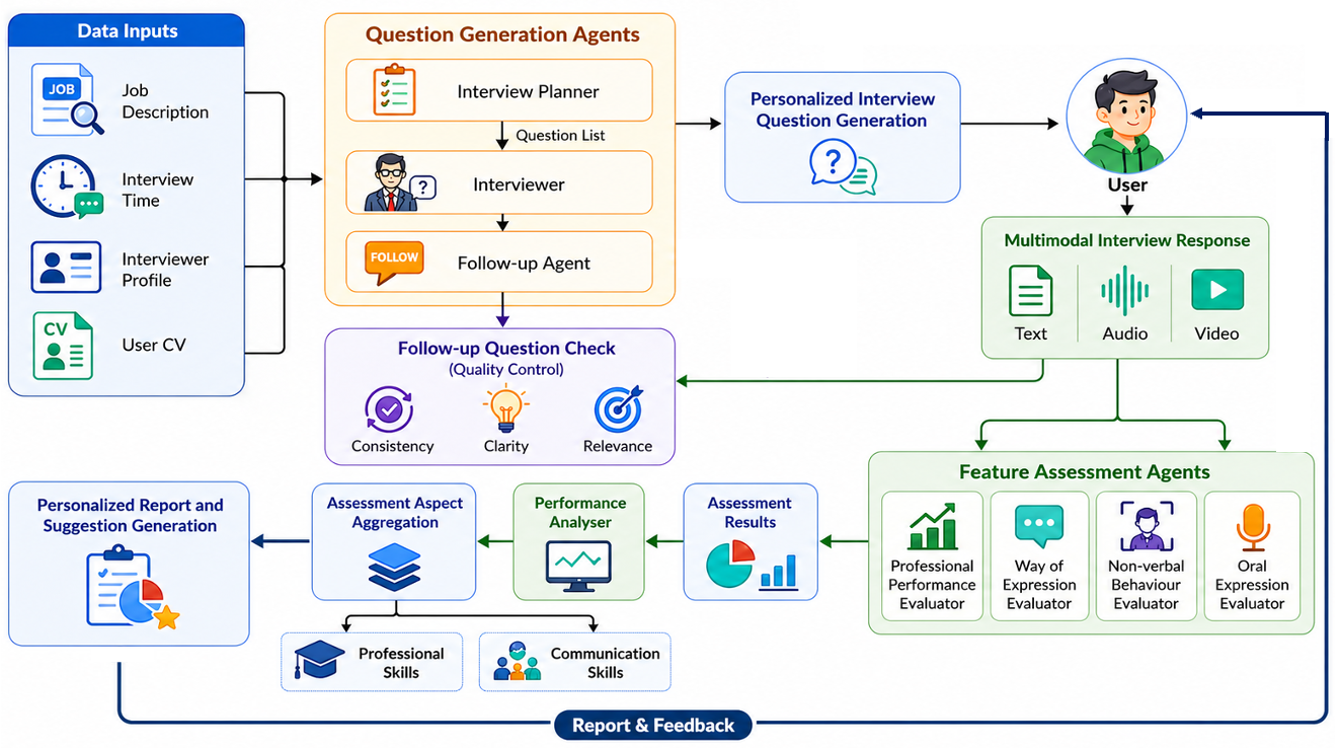
\includegraphics[width=0.88\textwidth]{figures/pipeline.png}
  \caption{The PolyInterview interview-simulation pipeline. Two questioning agents (Interview Planner and Interviewer) build a personalized session from the job description and CV; a follow-up check on each answer (consistency, clarity, relevance) gates further probing; four feature-assessment agents then score the answer across modalities, and the results are aggregated into a personalized report.}
  \label{fig:pipeline}
\end{figure*}

A session moves through setup, live interview, evaluation, and report (Figure~\ref{fig:pipeline}), driven by a multi-agent backend and a digital-human engine. From the student's side it is a short loop they can run at the live demo: configure one session, talk to the avatar, and read the report.

\paragraph{Setup.} On one screen the user picks an interviewer avatar, enters a company and position with its job description (or uploads one), uploads a CV (PDF/DOCX, parsed on the fly), and chooses an 8-, 15-, or 30-minute session, which the system maps to a question count. There is no prompt to write.

\paragraph{Embodied live interview.} The interviewer is a lip-synced digital human (Wav2Lip; \citealp{prajwal2020wav2lip}) streamed to the browser over WebRTC, with speech synthesis and streaming recognition for a spoken exchange; avatars differ in face, voice, and tone. Talking to a face restores the social pressure that flat-text practice cannot. Voice, expression, and posture stream in together and are recorded per question, so the system can later judge not just \emph{what} a candidate says but \emph{how}.

\paragraph{Multi-agent questioning (\textsc{Match}).} An \emph{Interview Planner Agent} reads the job description, interviewer profile, duration, and CV, and produces a structured question list spanning self-introduction, behavioral, skill-QA, and scenario stages. An \emph{Interviewer Agent} then asks each question in the chosen style and, after every answer, runs a Response-Check that rates consistency, clarity, and relevance and emits a follow-up signal: probe again, or move on. The three interviewer personas bind style to depth: Amy (Basic) asks at most one follow-up, David (Intermediate) two, James (Advanced) three, so the challenge scales with the candidate and personalization continues past the opening question. Ask a database candidate ``how would you keep a checkout fast under load,'' and a vague answer draws a follow-up on indexing while a crisp one is pushed toward consistency trade-offs.

\paragraph{Two-tier feedback.} After each answer, a per-question replay shows a 0--10 score, the transcript, a suggestion card (summary, strengths, fixes, a worked example), and a \emph{polished card} that applies targeted structural fixes (completing a missing STAR \emph{Result}, tightening terminology) to rewrite the candidate's own answer into a higher-scoring version with the same content, so the lesson is phrasing rather than new material. When the session ends, a whole-interview report integrates an overall verdict, the two competency scores, a radar over ten aspects, and a panel of thirteen multimodal features, and exports to PDF. The loop is deliberately pedagogical: each answer becomes the material for the next, better one.

\section{Explainable Multimodal Scoring}
\label{sec:scoring}

\begin{figure}[t]
  \centering
  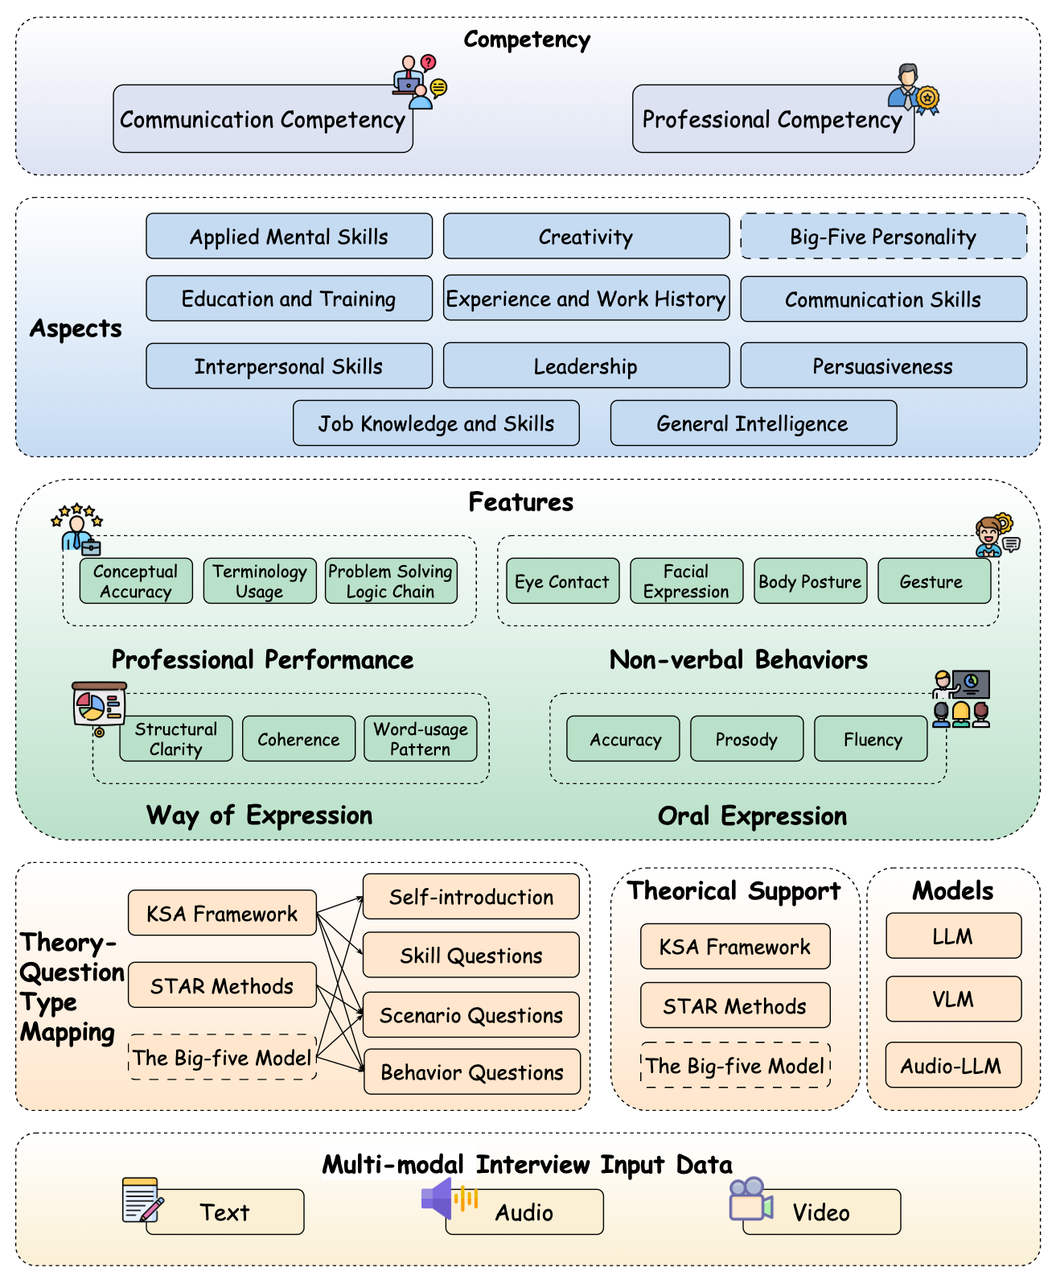
\includegraphics[width=0.92\linewidth]{figures/framework.png}
  \caption{The three-layer evaluation framework. Multimodal input (text, audio, video) feeds four feature agents that produce thirteen features; an aggregation step maps them to ten KSA-aligned aspects under question-type gating, and aspects roll up into two competency tracks. KSA, STAR, and the Big-Five model provide the theoretical grounding. Every score traces back across the layers to the behavioral signal that produced it.}
  \label{fig:arch}
\end{figure}

PolyInterview scores the \textsc{Convince} side with the three-layer architecture in Figure~\ref{fig:arch}. The four feature agents run concurrently (through a thread pool) on each answer, so per-answer scoring finishes within seconds and the final report is ready moments after the last answer, with no separate batch pass.

\paragraph{Layer 1 --- Features.} Thirteen 0--10 signals come from four agents that run together on each answer. A \emph{Professional-Performance} agent (LLM, text) rates conceptual accuracy, terminology use, and the problem-solving logic chain. A \emph{Way-of-Expression} agent (LLM, text) rates structural clarity, coherence, and word-usage pattern. A \emph{Non-verbal-Behavior} agent (vision-language model; \citealp{bai2023qwenvl}) rates eye contact, facial expression, body posture, and gesture from the recorded video. An \emph{Oral-Expression} agent (speech) rates pronunciation accuracy, prosody, and fluency from the audio.

\paragraph{Layer 2 --- Aspects.} An aggregation agent maps the features onto ten KSA-aligned aspects in three families: \emph{cognitive} (general intelligence, applied mental skills, creativity), \emph{background} (job knowledge and skills, education and training, experience and work history), and \emph{social} (communication, interpersonal skills, leadership, persuasiveness), the last aligned with the Big-Five factors \citep{mccrae1987validation}. Each aspect is a 70/30 weighting of primary and secondary features. Only the aspects \emph{relevant} to a question type are scored: a behavioral question activates interpersonal skills, applied mental skills, and leadership, while a skill-QA question activates job knowledge, general intelligence, and education. Teamwork is never scored on a question that cannot elicit it; the complete aspect--feature mapping and per-type gating are in Appendix~\ref{app:mapping}.

\paragraph{Layer 3 --- Proficiency.} Aspects roll up into Professional Competency (cognitive plus background) and Communication Competency (social), and the overall score is their mean; a CV-informed step tailors the improvement suggestions to the candidate's background.

\paragraph{Theory grounding.} Two established hiring frameworks keep the scores interpretable. KSA names \emph{what} we assess and drives the professional track; each K/S/A binds to a feature a language, vision, or speech agent can detect. STAR (Situation, Task, Action, Result) names \emph{how} a candidate should answer and drives the communication track, a structure with roots in behavior-description interviewing \citep{janz1982behavior}; a missing Result yields a concrete prompt to add one, and because students are scored against the structure they are taught, the feedback is directly usable. No score is a dead end: it traces from proficiency through aspect to the feature and modality that moved it.

\paragraph{Implementation.} The frontend is a Vue.js single-page app; a Flask API orchestrates interview flow and evaluation, and a separate Node/Express service handles authentication (Prisma + SQLite, bcrypt, JWT). Text scoring uses Qwen-Plus/Qwen-Flash via DashScope (switchable to GPT-4o through the OpenAI SDK); non-verbal analysis uses Qwen3-VL-Plus \citep{bai2023qwenvl}, streaming recognition uses a real-time Qwen3-ASR model, speech synthesis uses Edge-TTS (Azure backup), and pronunciation scoring uses the Azure Speech SDK. The digital human (LiveTalking + Wav2Lip) streams over WebRTC, and the platform runs as four cooperating services behind HTTPS with a session pool for concurrency.

\section{Deployment and What It Reveals}
\label{sec:deploy}

\begin{table}[t]\centering\small
\begin{tabular}{@{}p{0.67\linewidth}r@{}}
\toprule
\textbf{Statistic} & \textbf{Snapshot} \\
\midrule
Accounts & 101 \\
Returning accounts & 62 \\
Sessions & 1{,}564 \\
Generated questions & 7{,}665 \\
Completed sessions & 217 \\
Five-stage question sets & 1{,}422 \\
Distinct position titles & 83 \\
Answered question records & 1{,}274 \\
Recorded follow-up turns & 342 \\
Pooled scored answers & 1{,}425 \\
Audio/video files (wav/webm) & 1{,}744 / 1{,}754 \\
\bottomrule
\end{tabular}
\caption{All-account usage snapshot, including internal and test activity.}
\label{tab:deploy}
\end{table}


\paragraph{Deployment and corpus.} PolyInterview runs on the university network. The raw logs span 85 accounts and 1{,}535 sessions (14\,GB of text, audio, video, and CVs), but most of that volume is testing: a single \texttt{Test User} account holds 369 sessions, and integer-seed and junk accounts hold hundreds more. Four explicit rules (explicit ``test'' naming, internal integer-seed IDs, junk or placeholder names, and research-team self-tests) remove 39 accounts and leave \textbf{46 genuine users, 120 sessions, and 475 recordings} (Table~\ref{tab:deploy}); each answer is captured as WebM with an extracted WAV track of identical duration and is transcoded to MP4. We treat this cleaned set as ground truth and do not report the contaminated numbers, which tell a different and flattering story.

\begin{figure}[t]
  \centering
  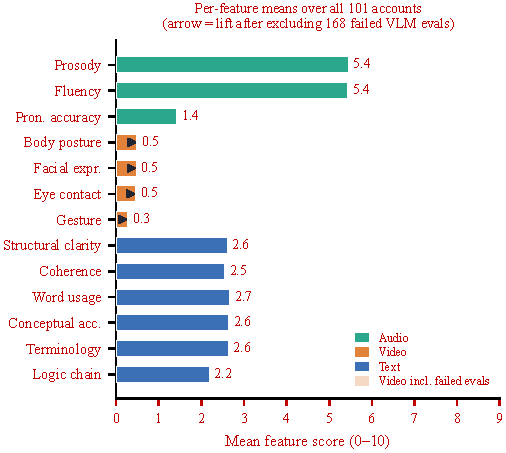
\includegraphics[width=\linewidth]{figures/fig_modality.pdf}
  \caption{Mean of each feature over the cleaned corpus, by modality. Audio (prosody, fluency) scores leniently high; text content sits near the floor on mostly short answers. For the four video features, the arrow marks the lift once the 74 hard-failures (silent zero-returns; Figure~\ref{fig:reliability}) are excluded; the 106 no-video answers are still counted, so this is a failure-only, conservative correction.}
  \label{fig:modality}
\end{figure}

\begin{figure}[t]
  \centering
  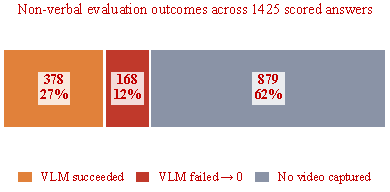
\includegraphics[width=\linewidth]{figures/fig_reliability.pdf}
  \caption{Outcomes of the non-verbal (video) evaluator across the 233 scored answers where it should have run. It silently returns a zero on 31.8\% of them; only 22.7\% yield a genuine score. The per-feature architecture is what makes this visible.}
  \label{fig:reliability}
\end{figure}

\paragraph{The architecture surfaces its own failure mode.} Because every score is traceable to a feature and modality, aggregating over the cleaned corpus does more than rank features; it audits the evaluator. Two things stand out (Figure~\ref{fig:modality}). First, audio features score leniently high (prosody and fluency near $6.6/10$) while text-content features sit near the floor, consistent with a corpus of mostly short, partly abandoned walk-up sessions (text content spans $0.76$--$1.12$; overall scores are zero-inflated, and among non-zero sessions the mean is only $1.76$ and the maximum $4.80$). Second, and more useful, the video features look low for a reason the architecture exposes: the non-verbal evaluator \emph{silently fails}, recording a zero, on $31.8\%$ of the $233$ answers where it should have run, with another $45.5\%$ having no usable video and only $22.7\%$ producing a genuine score (Figure~\ref{fig:reliability}). Excluding the failures lifts the video means by roughly $45\%$ (eye contact $1.11\!\rightarrow\!1.60$, posture $1.15\!\rightarrow\!1.66$). The headline ``vision scores lowest'' is therefore partly an artifact of unreliable inference on real, noisy webcam video---a diagnosis we could make only because each feature is reported separately rather than folded into one number.

\paragraph{Modalities carry non-redundant signal.} Across sessions, the modality scores are weakly related (text--audio $r{=}0.40$, text--video $r{=}-0.14$, audio--video $r{=}-0.10$), so the channels carry non-redundant signal and scoring all three is justified. The $31.8\%$ silent-failure rate is a separate matter: an engineering defect to fix at the source (retries, a fallback model, capture-quality checks), not something the other channels can paper over.

\section{Evaluation}
\label{sec:eval}
\paragraph{Pilot user study.} Across two rounds we gathered feedback from 129 participants spanning six institutions and eight-plus disciplines, including nine faculty reviewers from English-language teaching units. A broad first round endorsed the core experience (UI clarity 67\%, immersive digital interviewer 58\%, report depth 50\%, personalized questions 42\%), and deeper second-round interviews with senior students preparing technical interviews consistently reported that the flow was smooth enough for real practice, the questions felt professional and on-topic, and the digital interviewer felt close to a real session. These are self-reports, and we treat them as such.

\paragraph{Planned validation.} The deployment analysis points to what to measure next, and the explainable design makes each measurable. \emph{(i) Reliability.} We will report the non-verbal evaluator's failure rate as a first-class metric and drive it down with retries, a fallback model, and capture-quality checks; Figure~\ref{fig:reliability} is the baseline. \emph{(ii) Criterion validity.} We will collect blinded ratings from career-service experts on a stratified sample of recorded answers and measure agreement with the system per aspect (intraclass correlation and Krippendorff's $\alpha$), which the current self-report evidence cannot establish. \emph{(iii) Learning gain.} A pre/post design (a baseline mock interview, a block of PolyInterview practice, then a fresh interview scored by blinded experts) will test whether practice transfers, with an arm that toggles adaptive follow-ups to isolate their effect. These run in stages---reliability now, criterion validity next term, the learning-gain study after---alongside standardized usability and workload instruments (the System Usability Scale and Raw NASA-TLX) for active users, converting the system from ``well received'' to ``measured.''

\section{Conclusion}
PolyInterview is a deployed, multi-agent mock-interview system that pairs adaptive, personalized questioning with multimodal, theory-grounded, and traceable feedback. It is live, has served students across six institutions, and because every score points back to a behavioral signal, its own deployment data exposes where the evaluation is weak, starting with a non-verbal evaluator that fails silently on a third of answers. That traceability is the contribution we would most like reviewers and users to experience at the live demo: a score you can follow back to the moment that produced it.

\section*{Limitations}
The deployment evaluation is observational and self-reported; we do not yet report agreement between system scores and blinded expert ratings, which §\ref{sec:eval} is designed to fix. The cleaned corpus is modest (120 sessions, with a smaller effective sample once zero-score abandoned sessions are set aside), English-centric, and from a single institution, so the descriptive numbers should not be read as population estimates. The non-verbal failure rate we report is itself a moving target that depends on webcam quality and model availability. Finally, parts of the pipeline call external model providers under no-training terms; full on-campus inference is in progress.

\section*{Ethics Statement}
PolyInterview is an advisory practice tool for students, explicitly not a hiring or gatekeeping system, and its scores are explainable and contestable. Automated assessment of non-verbal behavior has a documented history of fairness concerns; we therefore keep visual scoring advisory, expose the evidence behind every score, avoid any pass/fail decision, and, as \S\ref{sec:deploy} shows, report rather than hide where that scoring is unreliable. Data is stored on the campus network with per-user isolation and bcrypt-hashed credentials and is deletable on demand; encryption at rest is on the deployment roadmap and not yet in place, which we state plainly. Any research use is de-identified and IRB-approved, consistent with GDPR and Hong Kong's PDPO; the analysis in this paper uses de-identified session metadata only.

\bibliography{references}

\appendix
\section{Aspect--Feature Mapping and Question Gating}
\label{app:mapping}
Every aspect score is a $70/30$ blend of primary and secondary features, so any score is reconstructable from the signals beneath it (Table~\ref{tab:mapping}). Only the aspects a question type can elicit are scored: \textbf{Self-Introduction} activates Communication Skills, Education \& Training, and Experience; \textbf{Behavioral} activates Interpersonal Skills, Applied Mental Skills, and Leadership; \textbf{Skill-QA} activates Job Knowledge, General Intelligence, and Education \& Training; \textbf{Scenario} activates Applied Mental Skills, Creativity, and Persuasiveness; \textbf{Candidate Questions} are not scored. As a worked example of traceability: when Professional Competency reads low, the report points to the feature that pulled it down---a Problem-Solving Logic Chain of $0.76$, say---while flagging a strong Prosody ($6.6$) as delivery that already works, so the student fixes answer structure rather than voice.

\begin{table}[h]
\centering\footnotesize
\setlength{\tabcolsep}{4pt}
\begin{tabular}{@{}lll@{}}
\toprule
\textbf{Aspect} & \textbf{Primary (70\%)} & \textbf{Secondary (30\%)} \\
\midrule
\multicolumn{3}{@{}l}{\emph{Cognitive}} \\
Gen.\ Intelligence & ConcAcc, Logic & Coher, Clarity \\
Applied Mental & Logic, ConcAcc & Clarity, Coher \\
Creativity & Logic, Word & ConcAcc, Coher \\
\midrule
\multicolumn{3}{@{}l}{\emph{Background}} \\
Job Knowledge & ConcAcc, Term & Logic \\
Education\,\&\,Train. & ConcAcc, Term & Clarity \\
Experience & ConcAcc, Logic, Word & Term \\
\midrule
\multicolumn{3}{@{}l}{\emph{Social}} \\
Communication & Clarity, Coher, Word & Eye, Face, Pron \\
Interpersonal & Eye, Face, Coher & Posture, Gest, Clarity \\
Leadership & Logic, Posture, Eye & Clarity, Face, Gest \\
Persuasiveness & Clarity, Coher, Word & Eye, Face, Prosody \\
\bottomrule
\end{tabular}
\caption{Primary/secondary features behind each aspect. Text features: ConcAcc (conceptual accuracy), Term (terminology), Logic (problem-solving logic chain), Clarity (structural clarity), Coher (coherence), Word (word-usage pattern); video: Eye, Face, Posture, Gest (gesture); audio: Pron (pronunciation accuracy), Prosody, Fluency.}
\label{tab:mapping}
\end{table}

\end{document}
